\section{question 1}

We want to solve the following equation for $F(t) = F_0 cos(\omega t)$:

\begin{equation}
	m \ddot{x}(t) + m \frac{\omega}{Q} \dot{x}(t) + m \omega^2 x(t) = F(t)
	\label{eq_diff}
\end{equation}
Equation \ref{eq_diff} is a second order linear differential equation. According to theorem 3.5.2 in Boyce \cite{Boyce}:
\begin{equation}
	x(t) = c_1 y_1(t) + c_2 y_2(t) + Y(t)
	\label{eq_x_1_emtpy}
\end{equation}

With $Y(t)$, any solution to the nonhomogeneous differential equation and with $y_1(t)$ and $y_2(t)$ that form a fundamental set of solutions to the homogeneous differential equation.
\begin{equation}
	\ddot{y}(t) + \frac{\omega}{Q} \dot{y}(t) + \omega^2 y(t) = 0
	\label{eq_diff_homo}
\end{equation}

We first solve $y(t)$ by seeing that, for constant values of $\omega$,$m$ and $Q$, a solution for equation \ref{eq_diff_homo} is  $y(t) = e^{r \: t}$. Applying to equation \ref{eq_diff_homo} yields:

\begin{equation}
	(r^2 + \frac{\omega}{Q} r + \omega^2) y(t) = 0 \; \; \Rightarrow \; \; r^2 + \frac{\omega}{Q} r + \omega^2 = 0
	\label{eq_characteristic}
\end{equation}

We find two solutions for r:
\begin{equation*}
	r_1 = - \frac{1}{2} \left( \frac{\omega}{Q} + \sqrt{\left( \frac{\omega}{Q} \right)^2 -4 \omega^2} \right) \; \; , \; \; r_2 = \frac{1}{2} \left( -\frac{\omega}{Q} + \sqrt{\left( \frac{\omega}{Q} \right)^2 -4 \omega^2} \right)
\end{equation*}

We use this to define:
\begin{equation*}
	y_1(t) = e^{r_1 t} \; \; , \; \; y_2(t) = e^{r_2 t}
\end{equation*}

$r_1$ and $r_2$ will be complex numbers for $\mid Q \mid > \frac{1}{2}$ meaning that differential equation \ref{eq_diff} will lead to a (damped) oscillator. Just as expected.\\
\\
The method to find $Y(t)$ is the method of undetermined coefficients described in section 3.5 of Boyce \cite{Boyce}.\\
We assume the $Y(t)$ is of the shape:

\begin{equation*}
	Y(t) = a_1 cos(\omega t) + a_2 sin(\omega t)
\end{equation*}

We find $a_1 = 0$ and $a_2 = \frac{F_0 Q}{\omega^2 m}$ (see appendix). Therefore we find:

\begin{equation*}
	x(t) = c_1 y_1(t) + c_2 y_2(t) + \frac{F_0 Q}{\omega^2 m}sin(\omega t)
\end{equation*}

By imposing the initial conditions on the latter result (see appendix) we obtain:

\begin{align*}
	c_1 = \frac{1}{r_2-r_1} \left( -\dot{x}_0 + \frac{F_0 Q}{\omega m} + x_0 r_2 \right)
\end{align*}
\begin{align*}
	c_2 = \frac{1}{r_2-r_1} \left( \dot{x}_0 - \frac{F_0 Q}{\omega m} - x_0 r_1 \right) \\
\end{align*}

We can plot $x$ as function of $t$ for the three discussed values of $Q$ (figure \ref{fig_q1}. For the sake of simplicity $\omega = 1$, $F_0 = 1$ and $m = 1$ in this plot. A scaled version of $F(t)$ is also plotted in the same axis in order to study the response of the oscillator with respect to driving force. 

\begin{figure}[h!] 
	\centering
	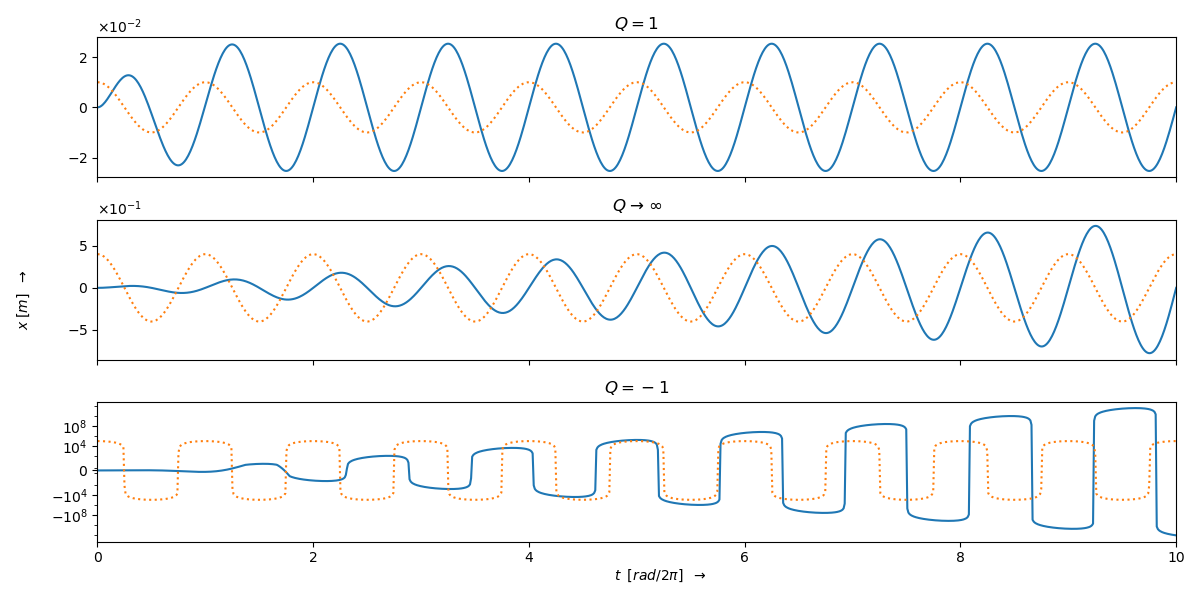
\includegraphics[width=0.6\textwidth]{figures/graph_q1.png}
	\caption{Graphs of $x(t)$ and $F(t)$  as function of $t$ for different values of $Q$. The solid blue lines correspond with $x(t)$ and the orange dashed lines correspond to a scaled version of $F(t)$.}
	\label{fig_q1}
\end{figure}

There are several conclusions that can be drawn from the graphs. For $Q = 1$, the oscillator will, after a period of amplification, oscillate with the same frequency as the driving force. However, with a phase shift. What's more, the oscillator seems to reach a steady state in approximately 1.5 oscillations where the amplitude stays constant. This steady state resembles a sine. The steady state is reached when the work done by the driving force on the system equals the energy dissipation by the friction. \\
For $Q \rightarrow \infty$ we find that the oscillator will also oscillate at the same rate as $F(t)$ but with a phase shift. However, the amplitude does not stabilize and seems to increase linearly with time. This makes sense since, considering that there is no friction ($Q \rightarrow \infty$), there is no energy dissipation in the system, only  work done on the system by the driving force. The system has the same frequency as the driving force so the energy gain by the system should be equal per oscillation. Therefore the oscillation amplitude, being directly proportional with the total energy in the system, should increase with the same amount each oscillation.  \\
For $Q = -1$ we find that the oscillator does not reach the same oscillating frequency as the $F(t)$. It seems to be lagging behind the driving force as a result of the 'negative friction' exerting a force in the same direction as the velocity. We also see that the amplitude of the oscillation increases linearly on a logarithmic y-scale. Therefore, the amplitude must increase exponentially with respect to time. This can be explained by the total energy in the system that gets amplified as a result of the 'negative friction'. 



 







